\documentclass{article}
\usepackage{amsmath}
\usepackage{amssymb}
\usepackage{graphicx}
\usepackage{cancel}
\usepackage{fitch}
\usepackage{tikz}
\usepackage{float}
\usepackage{caption}
\usepackage{wrapfig}
\usepackage{hyperref}
\hypersetup{
    colorlinks=true,
    linkcolor=blue,
    urlcolor=cyan,
    citecolor = red
}


% Keywords command
\providecommand{\keywords}[1]
{
  \small	
  \textbf{\textit{Keywords---}} #1
}


\title{The Physics of Spiritual Momentum}
\author{Carter Garrett}
\date{25 August 2024}

% TO DO: Find footnote insertion points for further reading. 
\begin{document}
    \maketitle

    \begin{abstract}
        In 2022, the Prophet and President of the Church of Jesus Christ of Latter Day Saints gave an address titled ``The Power of Spiritual Momentum \cite{Nelson}."
        The talk, given in the April General Conference session for that year, quickly became a focus point for the church member community. 
        President Nelson has given addresses in conferences prior wherein he has thematically employed words such as \textit{power} or \textit{rest}.
        In this paper, I will explore the physical relations between concepts President Nelson has cited in order to explore the full depth of the implications that remain undiscovered.
        As an effort to keep my \LaTeX \space skills sharp and gain more spiritual understanding, I present this document as a trivial review of proofs and public resource for future inquiry. 
        Source code is available in this \href{https://github.com/carter-mg/projects-assorted.git}{Git Repository}.
    \end{abstract}

    \keywords{Momentum, Newtonian Mechanics, relativistic momentum, power, energy, velocity}

\newpage

    \tableofcontents

\newpage

    \section{Physical Foundations}

        \subsection{Newtonian Momentum}

            \subsubsection{Mass}
                We begin by defining and investigating the Newtonian definition of momentum, as well as its exensions and relations, specifically with mass. 
                \par
                It is very easy to practially define mass. But conceptually, mass is a very obscure idea to capture.
                There exists a multiplicity of physical definitions for mass. Generally, it refers to the `stuff' of an object, or its substance. While seemingly simple, it becomes immediately complex-- how do you determine the quantity of that object's `stuff?' 
                \par
                Throughout history, humanity has associated mass with gravity and weight (the strange tendency of stuff to move together). The concept of weight is closely connected to mass, but not identical. 
                An object's \textit{weight} is generally defined as the force it experiences due to gravity. Newton understood that gravitational forces are proportional to mass,\footnote{$F = G\tfrac{M \cdot m}{r^2}$: As mass incrases, so does the gravitational attraction.}
                or in other words, if something has more mass, it experiences a greater force due to gravitational attraction.
                And by extension, if it experiences a greater force, it will \textit{weigh} more. Therefore, weight is actually a kind of a pointer for mass. 
                So, for example, if an object A weighs more on Earth than object B, we say it has more mass as in Figure \ref{fig:weigh}.
                
                \begin{figure}[H]
                    \centering 
                    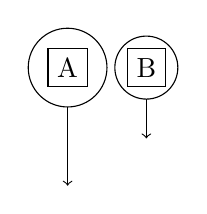
\begin{tikzpicture}
                        
                        \draw(0,0) circle (0.5cm);
                        \draw(1,0) circle (0.4cm);
                        \draw[->] (0, -0.5) -- (0, -1.5);
                        \draw[->] (1, -0.4) -- (1, -0.9);
                        \node[draw] at (0,0) {A};
                        \node[draw] at (1,0) {B};

                    \end{tikzpicture}
                    \caption{} \label{fig:weigh}
                \end{figure} 
            
                Force due to gravity, in Figure \ref{fig:weigh}, is represented by arrows. Because object A has more mass, it experiences a greater force. 
                Today, we define the kilogram as the standard unit of mass by weight. We have successfully found a way to quantitatively describe mass.\footnote{While this is principally the correct definition of mass, modern definitions include the numerical value of Planck's constant $h$, in combination with the meter as defined by the speed of light $c$ and the second as $\Delta \nu_{Cs}$. See \href{https://www.bipm.org/en/si-base-units/kilogram}{this page} for a full explanation.}
            
            \subsubsection{Inertia and Momentum}
                What if we want to know the mass of something that isn't found on Earth? This is a problem, because until now we have needed Earth's gravity to determine mass using the kilogram-- and we don't want our definition to have faulty contingencies. Mass is also often thought of in relation to \textit{inertia}, or its `resistance to acceleration \cite{Bray}.'
                Isaac Newton is acknowledged as the first to recognize that if something is not moving, it probably won't start moving again \cite{Newton}. If we were to take a ball and rest it on a table, it would stay put. This is Mr. Newton's first great kinematic law.
                Again, this seems like common sense. But in reality, this is a very interesting property of mass.
                \par
                If we take object A and object B again, we might imagine trying to move each by force. Most of us would intuitively suspect that object A would be more difficult to move.

                    \begin{figure}[H]
                        \centering
                        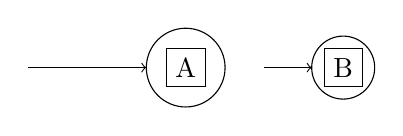
\begin{tikzpicture}
                            
                            \draw(0,0) circle (0.5cm);
                            \draw(2,0) circle (0.4cm);
                            \node[draw] at (0,0) {A};
                            \node[draw] at (2,0) {B};
                            \draw[->] (-2, 0) -- (-0.5, 0);
                            \draw[->] (1, 0) -- (1.6, 0);

                        \end{tikzpicture} \caption{}\label{fig:2}
                    \end{figure}                    

                As in Figure \ref{fig:2}, object A would greater resist the forces that attempt to induce motion. We can therefore say it has more mass! 
                \par
                This brings us to Mr. Newton's second kinematic law and the definition of inertial mass, and can be easily quantified \cite{Newton}! The force required to change an object's velocity (or to accelerate it) is \emph{proportionate to that object's mass}.

                \begin{equation}\label{eq:1}
                    F = m \cdot a
                \end{equation}
                \begin{center}
                    ($F$ representing force, $m$ and $a$ being mass and accelereation, respectively.)
                \end{center}
                
                Now suppose we apply a force to create velocity (or rate of change in position) in object A.
                If we wanted to stop it, we couldn't just `will' the ball to stop rolling by our minds. Unless it were by some incomprehensible physical processes, the ball could only stop rolling by force.
                
                Thus, the inertia of object A is defined as its property to resist any change of velocity unless by force-- it will not spontaneously change. Momentum, however, is defined as the `amount of motion' possessed. 
                This is inherently different than velocity. Recall that velocity is only the rate at which an object changes position over time.\footnote{This explanation includes references to the kinematic equations, which can be referenced on \href{https://byjus.com/physics/kinematics-equations/}{this web page}.} 
                The ball might be traveling with a velocity of one meter each second, but is not associated with the mass of the ball. `Amount of motion' refers to the velocity as well as the inertial mass of an object.
                
                Therefore, momentum, or the `amount of motion' is proportional to an object's inertial mass \emph{and} velocity. So an object has greater momentum (and is harder to start or stop moving) if it is really big or is moving really fast. 

                \begin{equation}\label{eq:2}
                    p = m \cdot v
                \end{equation}
                \begin{center}
                    ($p$ representing momentum, $m$ and $v$ representing mass and velocity, respectively)
                \end{center}

                We have successfully explored the derivation of Newtonian momentum.

            \subsubsection{Energy}
                An equally important concept that will be relevant later on is that of energy. An object's energy is its ability to do work.\footnote{Work is to apply a force in a manner that displaces the object. $W = F \cdot d$.}
                Interestingly enough, we also recognize energy to be heat or light. The idea can be traced back to Gottfried Leibniz,\footnote{A complete history of the development of the concept is messy. Newton, Chatelet, Young, Coriolis, and Joule, among many other scientsts contributed to its development. See \href{https://spark.iop.org/history-concept-energy-and-work}{this page} for more.} 
                who referred to an early form of the concept \cite{Smith}.
                There are many ways that energy can be identified, table \ref{tab:1} below contains the most prevalent.
                \begin{table}[H]
                    \caption{}\label{tab:1}
                    \begin{enumerate}
                        \item Kinetic Energy
                            \begin{description}
                                \item[$KE =\tfrac{1}{2}mv^2$] 
                                \item[Note:]$KE$ is proportional to velocity squared.
                            \end{description}
                        \item Gravitational Potential Energy
                            \begin{description}
                                \item[$PE = mgh$]
                                \item[Note:] $h$ is height, $g$ is acceleration due to gravity on Earth ($9.8 ms^{-2}$).
                            \end{description}
                        \item Electrical Energy
                            \begin{description}
                                \item[$E = P \cdot t$]
                                \item[Note:] $P$ is power, $t$ is time. 
                            \end{description}
                        \item Thermal Energy
                            \begin{description}
                                \item[$Q = mc\Delta T$]
                                \item[Note:] $Q$ being energy, $c$ being the object's specific heat capacity, and $\Delta T$ being the change in temperature. 
                            \end{description}
                        \item Work
                            \begin{description}
                                \item[$W = F\cdot d$]
                                \item[Note:]$F$ being force and $d$ being distance.  
                            \end{description}
                    \end{enumerate}

                \end{table}

                Energy is commonly measured in units of Joules, which can be manipulated many ways. The joule is easily expressed as Newtons (the standard unit of force) times meters (the standard unit of distance). 
                We can relate energy to momentum using the following work-energy relationship:
                
                \begin{equation}\label{eq:3}
                    \begin{split}
                    E & = N \cdot m \\
                    & = kg \cdot \frac{m}{s^2} \cdot m \\
                    & = kg \cdot \frac{m}{s} \cdot \frac{m}{s}\\
                    \end{split}
                \end{equation}
                \begin{center}
                    (Note that we have $m \cdot v \cdot v$)
                \end{center}
                \begin{equation}\label{eq:4}
                    \begin{split}
                    E & = \boxed{m \cdot v} \cdot v \\
                    & = p \cdot v \\
                    \end{split}
                \end{equation}

                Following equation \ref{eq:4} and taking the definition of kinetic energy from table \ref{tab:1}, you eventually obtain the common relations between Kinetic Energy and momentum:

                \begin{equation}\label{eq:5}
                    KE = \frac{p^2}{2m}
                \end{equation}
        
            \subsubsection{Power}
                While most often discussed in electrodynamics, power is important to review for our purposes as well. The most typical unit of power is the Watt (Joules per second).
                With the definitions of energy in place, power can be defined as energy over time:

                \begin{equation}\label{eq:6}
                    P = \frac{E}{t}
                \end{equation}
                \begin{center}
                    ($E$ being energy, $t$ being time in seconds)
                \end{center}

        \subsection{Non - Newtonian Momentum}
            The Newtonian model for kinematics and mechanics has worked wonderfully for centuries. However, especially in the last century, there have been discrepancies between Newtonian predictions and measured observations.
            Albert Einstein is well known for revolutionizing physics with his papers outlining special relativity and the mass-energy equivalence. These provided predictions that matched observations where Newetonian kinematics failed \cite{Einstein1}.\footnote{The most well-known example is the precession of Mercury's orbit.}
            We will circumnavigate a full justification of his theories in this paper.
            \par
            Suffice it to say that momentum does not apply accurately to objects moving at speeds non-trivial compared to the speed of light (we can't describe the momentum of things that are traveling \emph{really} fast with Newtonian momentum).
            Because Einstein postulated the mass - energy equivalence, he was able to produce what is known as relativistic momentum:

            \begin{equation}\label{eq:7}
                \begin{split}
                    p & = \frac{m_0v}{\sqrt{1 - \frac{v^2}{c^2}}} \\
                    & = \gamma m_0v \\
                \end{split}
            \end{equation}
            \begin{center}
                (Note that $\gamma = \dfrac{1}{\sqrt{1 - \dfrac{v^2}{c^2}}}$ is used to simplify)\footnote{This simplification is known as the Lorentz factor, commonly represented by $\gamma$. The Lorentz transformations are not discussed in this paper.}
            \end{center}

            Further, a relativistic object will have a total energy that is the Pythagorean Sum of its momentum and rest mass.

            \begin{equation}\label{eq:8}
                E^2 = (pc)^2 + (m_0c^2)^2
            \end{equation}

\newpage
        
    \section{Momentum and Spiritual Momentum}
            
        \subsection{Description of Spiritual Momentum}

            In order to successfully draw inferences between physical and spiritual momentum, we must understand how President Nelson describes it.
            Firstly, it is interesting to note that President Nelson encourages his audience to be peacemakers in all circumstances, and invokes the concept of spiritual momentum to help them do so \cite{Nelson}. 
            He remarks: 

            \begin{center}
                \textbf{\textit{``Momentum is a powerful concept. 
                We all have experienced it in one form or another— for example, in a vehicle that picks up speed or with a disagreement that suddenly turns into an argument."
                }}
            \end{center}

            President Nelson establishes that he is referring to the concept of momentum not only in the physical world, but as the same conceptual principles that apply to the sentimental or abstracted aspects of our lives.
            He continues by discussing the nature of spiritual momentum:

            \begin{center}
                \textbf{\textit{``So I ask, what can ignite spiritual momentum? We have seen examples of both positive and negative momentum... 
                We have never needed positive spiritual momentum more than we do now, to counteract the speed with whih evil and the darker signs of the times are intensifying...''
                }}
            \end{center}

            He attributes the impartial nature of physical momentum to spiritual momentum, but that positive \emph{spiritual} momentum is required for our day. 
            To instruct his listeners, he provides a list of five actions that will `fuel positive spiritual momentum:'

            \begin{enumerate}
                \item [1.] Get on the covenant path and stay there.
                \item [2.] Discover the joy of daily repentance.
                \item [3.] Learn about God and how He works.
                \item [4.] Seek and expect miracles.
                \item [5.] End conflict in your personal life.
            \end{enumerate}

            President Nelson ends by promising an increased capacity to accrue spiritual momentum. Besides this, he mentions very little explicitly about spiritual momentum in the address. 

            In other addresses, President Nelson mentions power in the following way \cite{Nelson2}: 

            \begin{center}
                \textbf{\textit{``God so loved the world that He sent His Only Begotten Son to help us. 
                And His Son, Jesus Christ, gave His life for us. 
                All so that we could have access to godly power— power sufficient to deal with the burdens, obstacles, and temptations of our day. 
                Today I would like to speak about how we can draw into our lives the power of our Lord and Master, Jesus Christ.''
                }}
            \end{center}

            He also describes a spiritual principle of rest \cite{Nelson3}: 

            \begin{center}
                \textbf{\textit{``The reward for keeping covenants with God is heavenly power... This power eases our way. Those who live the higher laws of Jesus Christ have access to His higher power.
                Thus, covenant keepers are entitled to a special kind of rest that comes to them through their covenental relationship wth God.''}}
            \end{center}

            So it appears that a consequence of spiritual power is spiritual rest. It is also crucial to add here that President Nelson defines this special spiritual form of rest as one that does \emph{not} absolve the holder of trial or obstacles. 
            
            Each of these concepts are profoundly associated with the physical concepts laid out earlier in this document.

        \subsection{Comparison of Spiritual and Physical Momentum}
            \subsubsection{Mass and Velocity in Momenta}
                We reroute to our foundational concept of mass. If we interpret President Nelson's comments correctly, we as agents are the objects that acquire spiritual momentum by fulfilling the five directives he provides.
                If the commission or omission of the directives increase or decrease spiritual momentum, then those are the corresponding 'forces' that operate on the mass.\footnote{The interjection is easily made that agents are not `acted upon' by exercising volition according to LDS theology. See 2 Nephi 2.}
                Importantly, in `omitting' to do as President Nelson commends, the agent is not inactive. A decision is made regardles, albeit in misalignment with President Nelson's counsel. 

                In the analogy, if mass is as the human agent, then it follows that spiritual momentum, as an intangible property, can be gained as force is applied in either a positive or negative manner.
                A very natural question arises: Are we, as spiritual mass-agents inertial? If we possess some form of impetuous \textit{vis viva} in any direction, will we maintain that course unless acted upon by some force?
                
                Spiritual stagnancy is often cited as a legitimate spiritual phenomenon in the Church of Jesus Christ of Latter-Day Saints. Progression can halt without action on the part of the agent. Therefore it may be argued that we, as agents, do not possess `spiritual inertia' as physical matter does. 
                Conversely, let it be said again that there is no such thing as spiritual inaction, and therefore agents are constantly affecting their aggregate spiritual momentum with every conscious and subconscious decision.

                Therefore, the analogy seems to hold best with the premise of `inertial spiritual mass' in place. Spiritual mass, for the purposes of our inquiry, will describe the intrinsic resistance to spiritual forces.\footnote{It is not desirable to imply an inherent inequality among the spiritual offspring of God. Although undesirable, it seems correct to say that each individual responds to spiritual influences differently}
                We now recall the formal physical definition of momentum (Equation \ref{eq:1}).

                \[p = m \cdot v\]

                We have assigned significance to $p$ and $m$, only $v$ remains. What is spiritual velocity? And what does it mean if a larger mass contributes to a greater spiritual momentum?
                
                If we hold velocity constant and allow mass to vary, then it follows that an individual's response to spiritual forces may be large or small. 
                Large `spiritual masses' at rest may respond with a smaller change in velocity when a force of some value acts upon it.\footnote{Impulse is a physical concept defined by $\Delta p = F \Delta t$. A change in momentum is proportional to a force exerted over time.}
                Small `spiritual masses' at rest may respond with a greater change in velocity when a force of the same value acts upon it.
                In essence, this is to say that the large mass moving slower will have the same momentum as the small mass moving quicker. 

                In pursuit of the analogy, a large spiritual mass may experience difficulty in gaining velocity, but will not stop easily. 
                On the contrary, a small spiritual mass may easily obtain a large velocity, but can easily be stopped. 
                This seems right-- some individuals experience an erratic spiritual journey with many changes in velocity, and others experience a slowly accelerating journey of consistency.
                It cannot be said at this stage, whether one is more preferrable than the other.

                Now, concerning the idea of spiritual velocity. The easiest comparison is `the rate of change in spiritual position.' This makes enough sense, but is subject to debate.\footnote{Scriptures can be cited in support or opposition of this claim, such as James 4:8 or Psalms 145:18}
                Velocity is ubiquitously defined as a vector quantity. This means that velocity is \emph{directional}, and not a scalar magnitude. Velocity includes how fast and in which direction an object changes its position.
                Again, this seems spiritually intuitive. The scriptures discuss the process of coming to God and spiritual momentum, as it is a vector quantity too, may bring us towards or away from God. 

                A formal definition then, might be: 
                
                \begin{center}
                  
                    \textbf{Spiritual Momentum}: The impetus or `amount of spiritual motion' an agent possesses, given by
                    \[p = m\cdot v\] 
                    where $m$ is spiritual mass and $v$ is spiritual velocity.

                    \textbf{Spiritual Mass}: The inertial resistance to spiritual forces. No standard units are given.

                    \textbf{Spiritual Velocity}: The rate of change in spiritual position, with respect to God. No standard units are given.
                    
                \end{center}
                
                We can adequately advance our inquiry into new physical domains. 

            \subsubsection{Spiritual Momentum and Energy}
                The objective of this section is to apply the relations established previously, between momentum, energy, and power, to spiritual momentum, energy, and power.
                While there is very much to be explored concerning spiritual energy, much has already been inspected by Aaron D. Franklin \cite{Franklin}. We will abandon some considerations for the intent of avoiding redundancy.

                Nonetheless, we articulated Equation \ref{eq:5} as a valid relationship between kinetic energy and momentum.

                \[KE = \dfrac{p^2}{2m}\]

                Understanding the spiritual intuition is convoluted. But this was derived from Equation \ref{eq:4}.

                \[E = p\cdot v\]
                
                This is more manegeable. It might be understood as `energy is the product of momentum and velocity.' Notice this is very close to the relativistic $E = pc$ expression.
                Is spiritual energy the product of spiritual momentum multiplied with spiritual velocity? The answer hardly seems clear. 
                If viewed relativistically, via the Pythagorean Sum of momentum and rest mass, we might find clarity. Recall Equation \ref{eq:8}.

                \[E^2 = (pc)^2 + (m_0c^2)^2\]

                This may be understood as: ``Total spiritual energy of an individual is equivalent to her Pythagorean Sum of relativistic spiritual momentum and spiritual rest mass.''
                 
                Now to grossly oversimplify: Because mass and energy are equivalent in special relativity,\footnote{Postulatd by Albert Einstein in Special Relativity, the famous $E = mc^2$. All objects, even at rest, possess an intrinsic energy. This concept is profound beyond the scope of this paper.} 
                total energy of any object must be the sum of whatever mass that object has at rest (rest mass) and the motional energy (kinetic energy).
                Thus, by virtue of volitional agents being spiritual masses, they possess an intrinsic energy that is equivalent to their rest mass. 
                Implicitly, total spiritual energy would increase with greater momentum and greater rest mass. It seems then, that greater spiritual energy is available to agents with greater rest mass.\footnote{Rest mass and inertial mass are subtly distinct concepts, but can be numerically equivalent. We circumvent exploring the nuances in this section.}

                Moreover, velocity affects total spiritual energy when an object is moving at relativistic speeds, or when $\tfrac{v}{c} \gg 0$.\footnote{Relativistic considerations typically apply when an object moves at $0.1c$, however appreciability varies by situation.}
                Recall Equation \ref{eq:7}. 

                \[p = \dfrac{m_0v}{\sqrt{1 - \frac{v^2}{c^2}}}\]

                By analysis, the faster an object travels in comparison with the speed of light, momentum becomes multiplicatively larger. 
                Continued manipulation of relativistic energy relations allows us to show that:

                \begin{equation}\label{eq:9}
                    \vec{v} = \dfrac{\vec{p}}{\sqrt{(mc)^2 + (\vec{p})^2}}c
                \end{equation}

                This indicates that the only instance in which an object can travel at the speed of light is when it is \emph{massless}.\footnote{A full demonstration is available on the \href{https://physics.stackexchange.com/questions/289034/reason-why-only-massless-particles-can-travel-at-speed-of-light}{Physics Stack Exchange Thread}. Sean E. Lake is credited with the best answer.}
                What does this mean metaphorically? Christ is scripturally recognized as 'the light' (Doctrine and Covenants 88:11 - 12). He is therefore spiritually massless and we, by consequence, are spiritually massive.
                Therefore we are incapable of travelling at Christ's lightspeed. 
                While impossible to travel at Christ's standard of $c$, if our spiritual velocity approaches $c$, we gain much more spiritual energy and momentum.\footnote{See Further Reading for more information.}

            \subsubsection{Power and Spiritual Power}
                Expanding on the definition of power (Equation \ref{eq:6}) as energy over time, power will now be examined spiritually.
                
                \[P = \dfrac{E}{t}\]

                By inspection, power can become greater with either an increase in energy or a reduction of time. President Nelson invited his audience to draw on God's power, or energy invested over time, by doing the following \cite{Nelson2}:

                \begin{enumerate}
                    \item[1.] Keep heavenly covenants.
                    \item[2.] Live the higher laws of Jesus Christ.
                    \item[3.] Reach up, as the woman with the issue of blood (Luke 8:44).
                    \item[4.] Invest time learning about the Savior and His Atonement.
                \end{enumerate}

                It is worth stating that power is sometimes described as something agents possess (Doctrine and Covenants 58:28) or something that agents are conduits of (Ether 12:2). 
                To draw God's power into one's life, then, is to seek an increase in spiritual energy or to decrease the time in which one unit amount of energy is received. 
                The suggestions listed by President Nelson either increase the quantity of spiritual energy in our lives (item 2), or decrese time in which we experience the same amount of God's energy (item 4).
                We risk disorienting ourselves by scrutinizing over details in the analogy. However, one important insight can be gained by considering the connection between power and energy.
                Recall Equation \ref{eq:6} and item 5 in Table \ref{tab:1}.
                \begin{equation}
                    \begin{split}
                        P & = \dfrac{E}{t}\\
                        & = \dfrac{F \cdot d}{t}\\
                    \end{split}
                \end{equation}
                \begin{center}
                    (Substituting work as a form of energy)
                \end{center}
                \begin{equation}
                    \begin{split}
                        P & = \dfrac{m \cdot a \cdot d}{t}\\
                    \end{split}
                \end{equation}
                
                Or, power is a product of spiritual mass, spiritual change in velocity, spiritual distance travelled, per unit time.
                To further abstract, agents gain spiritual power as they \emph{increase} their spiritual mass (increase $m$), increase the rate at which they come to God (increase $a$), take greater spiritual strides (increase $d$), all the more frequently (decrease in $t$)!
                
            \subsection{Rest and Spiritual Rest}
                This portion will not be fully elaborated, but it is an important part of our inquiry.
                In section 2.1, spiritual rest was defined as one that does not absolve the holder of trial or obstacles. 
                In physics, rest is understood as a motionless state \emph{relative to the observer's frame of reference}. This is to say that an observer on a plane would determine the seat in front of them to be at rest. 
                The observer's frame of reference is in motion identical to the plane. However, to an observer external to that motional frame, the plane and all of its contents would not be in a state of rest.

                Therefore, spiritual rest is not freedom from spiritual motion. The kind of spiritual rest that Christ offers (Matthew 11:28) \emph{includes} pains, sorrows, and afflictions. The joy associated with the rest, is far more valuable. 
\newpage

    \section{Additional Commentary}
            \subsection{Points of Discrepancy in Interpretation}
                With all of this said, we are hasty to comment that no choice of interpretation in analogies concerning spiritual momentum will be totally accurate. 
                There are many problems when moving from Newtonian foundations to a Relativistic setting, very little of which was explicitly mentioned in this document. 
                What's more, we lack a complete underestanding of concepts like spiritual power and energy. These are used in scripture to refer to God's dealings with His children, but are rarely ever fully defined. 
                This could result in errors within this document.

            \subsection{The Mark Dilemma}
                In Jacob 4:14, a `blindness' can come from `looking beyond the mark.' The concept of spiritual momentum was not intended to be the central point of President Nelson's address, and therefore a full development of the concept was not given.
                This could potentially result in errors within this document.

            \subsection{Inconsistent Terminology Problems}
                The theology of the Churh of Jesus Christ of Latter-Day Saints recognizes that prophets and scriptural canon are imperfect. 
                It is unreasonable to expect that authors of scripture as well as modern day prophets and revelations will be technically accurate and formally consistent with their choice of terms. 
                Therefore, in exploring President Nelson's comparison, we should not expect to find a perfect conceptual congruence.
                This may be the cause of potential errors in this document.

            \subsection{Further Reading}

                In this section, I will provide resources for readers to explore further possible connections to be made.

                \subsubsection{Christ as the Light and Special Relativity}
                    One of the foundational elements of special relativity is that the speed of light is constant in all reference frames. 
                    Formally, 
                    
                    \begin{enumerate}
                        \item [1.] The speed of light in a vacuum is the same for all observers regardless of the motion of light source or observer \cite{Jackson}.
                    \end{enumerate}

                    Setting aside dicussions concerning non-Euclidian spacetime and Minkowski space, the Lorentz transformations\footnote{For more information, see \href{https://en.wikipedia.org/wiki/Lorentz_transformation}{this page}.}
                    allow us to define what are known as `spacetime intervals.' In Galilean relativity, space and time are independent and separate events. However, in special relativity, time and space are \emph{fundamentally fused} informational elements.
                    Consequences of this phenomenon include the \href{https://en.wikipedia.org/wiki/Relativity_of_simultaneity}{destruction of simultaneity}, \href{https://en.wikipedia.org/wiki/Time_dilation}{time dilation}, and \href{https://en.wikipedia.org/wiki/Length_contraction}{length contraction}, among many others.
                    
                    It is very intriguing to consider the nature of spacelike, timelike, and lightlike intervals with respect to Christ as the light. Interesting relationships between causality and light arise. 

                    \begin{wrapfigure}{R}{0.5\textwidth}
                        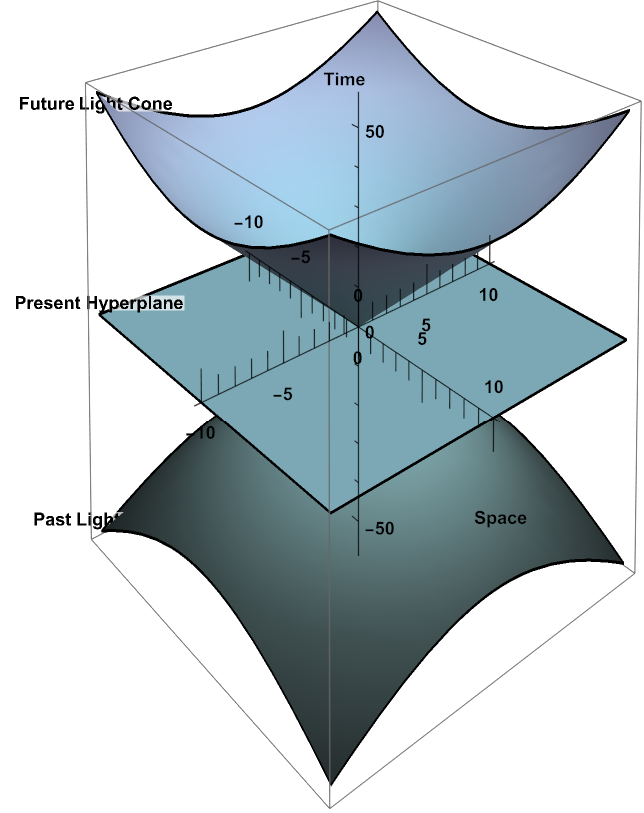
\includegraphics[scale = 0.4]{lightcone.png}
                        \caption{A visual representation of spacetime intervals, given by $\Delta s^2 = -(c\Delta t)^2 + \Delta x^2 + \Delta y^2 + \Delta z^2$.}
                    \end{wrapfigure}\label{fig:3}

                    Understanding how light bridges \emph{causal} relations between events could yield profound insights into the way we understand Christ as the light.
                    In Figure \ref{fig:3}, a common demonstration of light connecting spacetime geodesics is presented. The source code is listed below for reader's convenience and manipulation:
                    
                    \begin{center}
                        (In modified Wolfram Input syntax)
                    \end{center}
                        future[x\_, y\_]:= $\sqrt{\tfrac{x^2}{1} + \tfrac{y^2}{1}} \cdot 4$
                        
                        present[x\_]:= x

                        plot = Plot3D[
                            
                        \{future[x,y], -future[x,y], present[0]\}, 
                        
                        \{x, -10, 10\}, \{y, -10, 10\},

                        AspectRatio $\rightarrow$ Full, Mesh $\rightarrow$ None, ColorFunction $\rightarrow$ ``AtlanticColors", 
                        PlotLabels $\rightarrow$ Placed[\{``Future Light Cone",``Past Light Cone", ``Present Hyperplane"\}, \{Top, Bottom, Above\}], 
                        AxesOrigin $\rightarrow$ {0, 0, 0}, AxesLabel $\rightarrow$ {``Space", None, ``Time"}, 
                        AxesStyle $\rightarrow$ Black , LabelStyle $\rightarrow$ Directive[Bold, Medium], 
                        ViewPoint $\rightarrow$ {1.3, -2.4, 2.}
                        ]

                \subsubsection{Church Scholars on Light and Momentum}
                    Most material that is connected to topics covered here is contained in Aaron D. Franklin's book on the Spiritual Physics of Light \cite{Franklin}. 
                    However, many other church figures and scholars have referenced these ideas.

                    \begin{enumerate}
                        \item [1.] ``Spiritual momentum is created `over a lifetime as we repeatedly embrace the doctrine of Christ.' 
                        Doing so, President Russell M. Nelson taught, produces a `powerful virtuous cycle.' 
                        Indeed, the elements of the doctrine of Christ— such as faith in the Lord Jesus Christ, repentance, entering a covenant relationship with the Lord through baptism, receiving the gift of the Holy Ghost, and enduring to the end— are not intended to be experienced as one-time, check-the-box events. 
                        In particular, `enduring to the end' is not really a separate step in the doctrine of Christ— as though we complete the first four elements and then hunker down, grit our teeth, and wait to die. 
                        No, enduring to the end is repeatedly and iteratively applying the other elements of the doctrine of Christ, creating the `powerful virtuous cycle' that President Nelson described \cite{Renlund}.''

                        \item[2.] ``As I pondered how to maintain my positive spiritual momentum, I remembered an experience I’d had in Jerusalem. 
                        My first Sunday there, we attended the BYU Jerusalem Center for church. A student studying there gave a talk. 
                        She shared that when she’d first come to Jerusalem, she’d thought she would feel the Spirit so strongly all the time. She’d assumed that since she was walking where Jesus had walked, her testimony was going to be effortlessly strengthened.

                        Through her time there, she came to realize that it wasn’t about walking where Jesus had walked— it was about walking with Him \cite{Wood}.''

                        \item[3.] ``President Russell M. Nelson said: `I plead with you to let God prevail in your life. Give Him a fair share of your time. 
                        As you do, notice what happens to your positive spiritual momentum.' 
                        When I consciously choose to have faith in Jesus Christ every day and make time for those spiritual habits that connect me with Him, I remember my spiritually defining moments and feel a renewed sense of purpose, hope for the future, and faith \cite{Anonymous}.''
                    \end{enumerate}
                    
                    Most of these references have occurred in the Liahona Journal published by the Church of Jesus Christ. Their \href{https://www.churchofjesuschrist.org/?lang=eng}{webpage} will provide many references to the concept of spiritual momentum in the page search query. 

                    The author was surprised by the infrequency of references to the concept in official publication.

                \subsubsection{The Quantum Momentum Operator}
                        In quantum mechanics, the momentum operator is a linear differential operator. It is defined within a basis of Hilbert space which consists of momentum eigenstates. 
                        This branch of physics deviates significantly from the bases outlined in this paper, therefore, only resources for further inquiry will be provided.

                        \begin{enumerate}
                            \item [1.] Reading on the construction and derivation of the momentum operator\cite{Res.etal}.
                            \item [2.] A \href{https://quantummechanics.ucsd.edu/ph130a/130_notes/node102.html}{URL} with a brief explanation from the University of California San Diego and Jim Branson.
                            \item [3.] A mid-derivation \href{https://phys.libretexts.org/Bookshelves/Quantum_Mechanics/Introductory_Quantum_Mechanics_(Fitzpatrick)/03\%3A_Fundamentals_of_Quantum_Mechanics/3.06\%3A_Momentum_Representation}{mathematical explanation} from Richard Fitzpatrick at the University of Texas at Austin.
                        \end{enumerate}
\newpage
    \section{Concluding Remarks}
    The investigation of the physical notions surrounding spiritual momentum has proven to be, at the very least, interesting. The insights developed have been inspiring, and I hope that they can be refined as time continues. 
    Overall, the endeavor of writing this paper has, on many occasions, been reminiscent of a book written by Stephen C. Meyer. He received his Ph.D. in the philosophy of science from Cambridge. He is the author of ``Return of the God Hypothesis\cite{Meyer},'' which is a review of the scientific history and current status of the God Hypothesis.
    It represents his attempt to prove that in the age of New Atheism, the God Hypothesis has not been totally overcome. Though this paper does nothing to comment or contribute to that argument, it is my insufficient effort to blend science and religion in a new way.
    I express my gratitude to those who have received this well and engaged with the ideas I present.
\newpage

    \nocite{*}
    \bibliographystyle{plain}
    \bibliography{refs}

\end{document}